\documentclass[10pt, a4paper]{article}
\usepackage{fullpage}
\usepackage{graphicx}
\usepackage{subcaption}

\DeclareGraphicsExtensions{.jpg, .png, .pdf} %.jpg .png .pdf

\setlength{\parskip}{0.2cm}
\setlength{\parindent}{0cm}
\addtolength{\textheight}{25pt}

\begin{document}
\title{Product Management
\\ 3D Heap Visualisation}
\author{Aviv Beeri, Briony Goldsack, Ying Jiang, Oliver Myerscough,
\\ Anna Thomas, Eleanor Vincent}
\maketitle


\section{Introduction}

An object-oriented software application creates complex structures on the heap during its lifetime. Debugging object-oriented software often involves thinking about how the heap evolves as a program runs. The aim of our group project is to design a tool which supports visualisation of the heap of a running Java program as a 3D scene which can be navigated by the software developer by moving around as if in a first person shooter game.

This report aims to present the methods we have employed to elicit and manage the requirements of our project. We will discuss our stakeholders, how we have prioritised the requirements and decided what to build and how we plan on testing whether we have built the right product. 

\section{Customers and Stakeholders}

In our project we have a variety of types of customers, the first being our internal customer\textsuperscript{\cite{internal,internal2}} and project supervisor Alistair Donaldson. As our supervisor he is directly connected to the project and we have a close working relationship with him. Weekly meetings are organised to keep him updated on the project so we can acquire useful feedback from him on the latest features to adjust the product according to his advice and interests. These meetings are also useful to discuss what features should be implemented next and prioritised. It is important to maintain good relations and constant feedback from internal customers so that we can continue to rely on their expertise and advice throughout the project (As shown in the feedback section).

We have also targeted our 3D heap visualisation tool directly at a variety of consumers whom we feel would benefit from using our product. These consumers can be other students, programmers or gamers. Interacting with our consumers is a key part of ensuring we are building the right product, as part of our consumer base are students we can easily gain feedback from other university students on our course and in lab sessions.

Aside from the eventual users of the product there are many other stakeholders\textsuperscript{\cite{stakeholder}} to consider, for example, once our project is complete if it was being used by students in the university then it would be necessary to keep the software up to date and fix any bugs found. Therefore maintenance staff would be stakeholders, this means that our code must be maintainable and well documented so someone who hadn’t worked on the project would be able to understand and fix it. If the product was used as a teaching tool then lecturers, laboratory helpers and students would need to be able to install and operate the system so the product would need to be accessible and usable by them.

\begin{figure}[h]
        \centering
        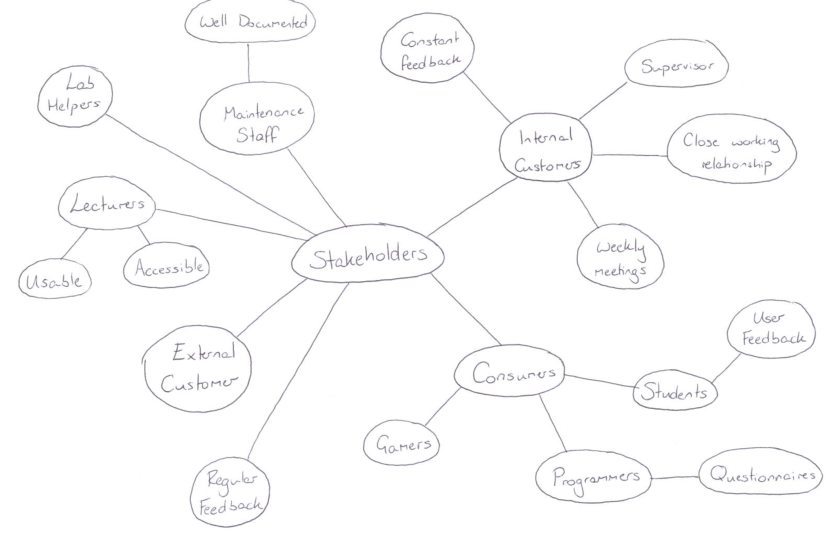
\includegraphics[width=250px]{images/stakeholders.png}
        \caption{Stakeholders}
\end{figure}

\section{Requirements}

\subsection{User stories and Personas}

Extreme programming introduced the practice of expressing requirements in the form of user stories to describe the desired functionality of the system from the perspective of the customers. User stories have allowed us to be precise in our requirements by presenting them at a high level, smoothing out complexity, and exploring the customers behind them through personae.  Another advantage of using user stories is that they can be written and then replaced with more detailed stories when necessary\textsuperscript{\cite{mikeadv}}. Though one disadvantage is that it is difficult to encompass all of a system’s requirements in this form. 

Our first step in creating user stories was to envision our end users (actors within each use case). We identified three initial applications of our heap visualisation tool which gave us an insight into our ‘actors’:
\begin{itemize}

  \item Teacher/Lecturer
  \item Beginner Programmer
  \item Experienced Programmer 
  \item A Typical Gamer 

\end{itemize}
We decided to combine the agile development user story strategy with methods introduced in the HCD course in the form of personae (fictional people and their requirements for the product) to allow us to imagine in more detail scenarios in which our heap visualisation tool could be used.

\begin{figure}[h]
        \centering
        \begin{subfigure}[b]{0.4\textwidth}
                \centering
                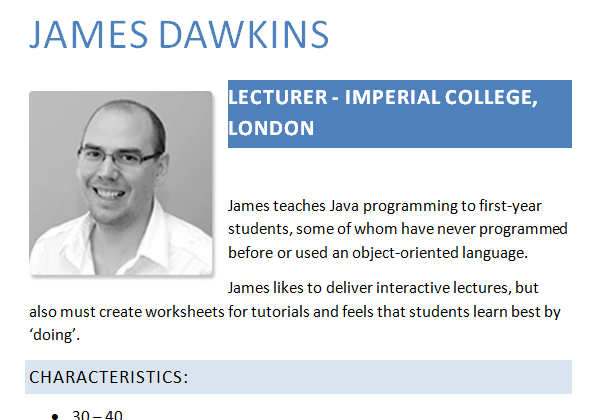
\includegraphics[width=100px]{images/Persona_1.png}
                \caption{Persona One}
        \end{subfigure}
        \quad %add desired spacing between images, e. g. ~, \quad, \qquad etc.
          %(or a blank line to force the subfigure onto a new line)
        \begin{subfigure}[b]{0.4\textwidth}
                \centering
                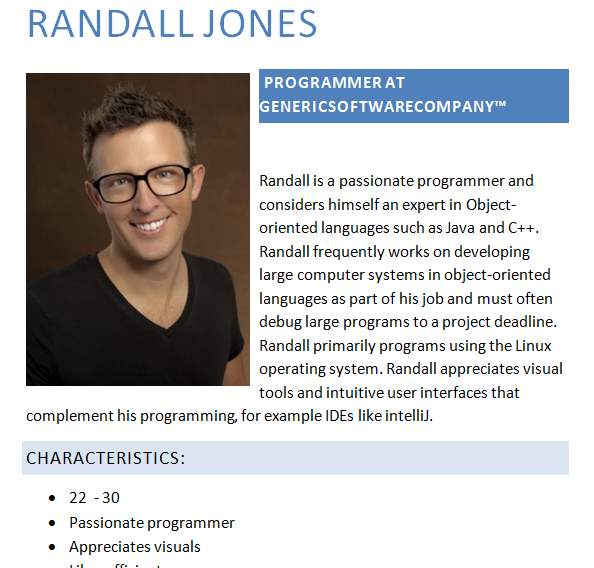
\includegraphics[width=100px]{images/Persona_2.png}
                \caption{Persona Two}
        \end{subfigure}
        \quad
        \begin{subfigure}[b]{0.4\textwidth}
                \centering
                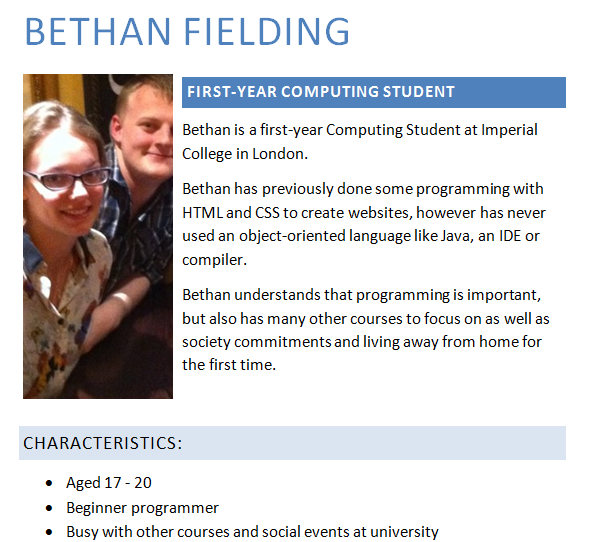
\includegraphics[width=100px]{images/Persona_3.png}
                \caption{Persona Three}
        \end{subfigure}
        \quad
        \begin{subfigure}[b]{0.4\textwidth}
                \centering
                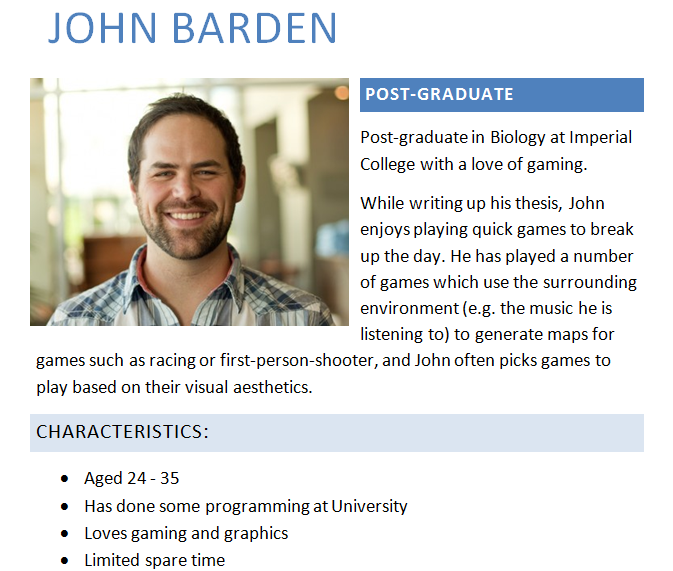
\includegraphics[width=100px]{images/Persona_4.png}
                \caption{Persona Four}
        \end{subfigure}
        \caption{}
\end{figure}

Following on from these personae, we were able to create user stories for each group of potential customers. In some cases, these user stories began quite general, but were developed to be more specific as the project progressed. 

\subsubsection{User story examples:}
\begin{itemize}
  \item “As a lecturer in Computer Science, I want to visualise the references created using polymorphism as an aid to teaching object-oriented languages.”
  \item “As a lecturer in Computer Science, I want to demonstrate garbage collection strategies as an aid to teaching object-oriented languages.”
  \item “As an experienced programmer, I want to visualise memory usage to assist in debugging a program.”
  \item “As a novice programmer, I want to visualise object information in order to learn more about the information stored on the heap.”
  \item “As a gamer, I want to visualise the heap as a 3D interactive world so that I can complete dynamically-generated missions.”
\end{itemize}


\subsection{Prioritising requirements}

Having carried out our use case analysis, we identified a set of base requirements, which we felt were essential to the project, as well as a set of requirements which could be added if time permitted. We prioritised our requirements base upon our user stories. Many of our user stories had features in common so formed our fundamental requirements. Priorities for additional requirements were focused around our customers. Most important of whom was our internal customer who had commissioned the project. Hence, primarily we wanted our tool to be educational.

\subsection{Managing requirements}

It is customary that a user story is implemented in a single iteration of an agile project. Most of our stories have worked well, for example, depicting the references within the 3D world from object to object. However, there have been some stories for which we have had to split the story over multiple iterations. For example, the creation of the interactive 3D landscape as a visually appealing entity that can be updated in real-time as a program runs. We decided to split this particular story up into a series of smaller stories by dividing the features of the 3D world into high priority that should be done first (as other stories depend upon it) and other parts that could be left until later. That is to say we created additional, more-developed user stories following an imaginary flow of user actions when using our tool, containing the goals:
\begin{itemize}

  \item I want to visualise the heap in 3D
  \item I want to walk around the 3D world
  \item I want to interact with the objects in the 3D world
  \item I want the world to be visually appealing 

\end{itemize}
We then divided these by priority. Namely that the 3D rendering and interactivity were of high priority and the attractive graphics could be put off until later. Splitting up stories in this way is better than splitting up the stories depending on the kind of work that needs to be done or the application layers that are involved (horizontal slicing) for several reasons\textsuperscript{\cite{eight}}. Firstly, individual items such as the back-end of the debugger or the front-end of the GUI do not provide value separately, and so do not contribute to agile development as we may not always have a releasable product. Furthermore, splitting the work in this way could lead to bottlenecks, for example, the person in charge of designing the user interface may not get their work done on time so it cannot be integrated with the debugger. Another disadvantage is that so-called horizontal slices cannot be prioritised as they are all essential to the final product.  

\section{Development}

\subsection{Paper Prototypes}
 	
In a design process, paper prototyping is one of the fastest techniques and offers opportunity for designers to collect usability data as early as possible which in turn reduces potential risks in later stages. It is also cheaper to make changes to the product in early stage than later. Furthermore, prototyping involves early communication with stakeholders and get feedback from them. For our project, we need a user interface. Before actually coding the user interface on a computer, we drew a paper prototype of GUI.

\begin{figure}[h]
        \centering
        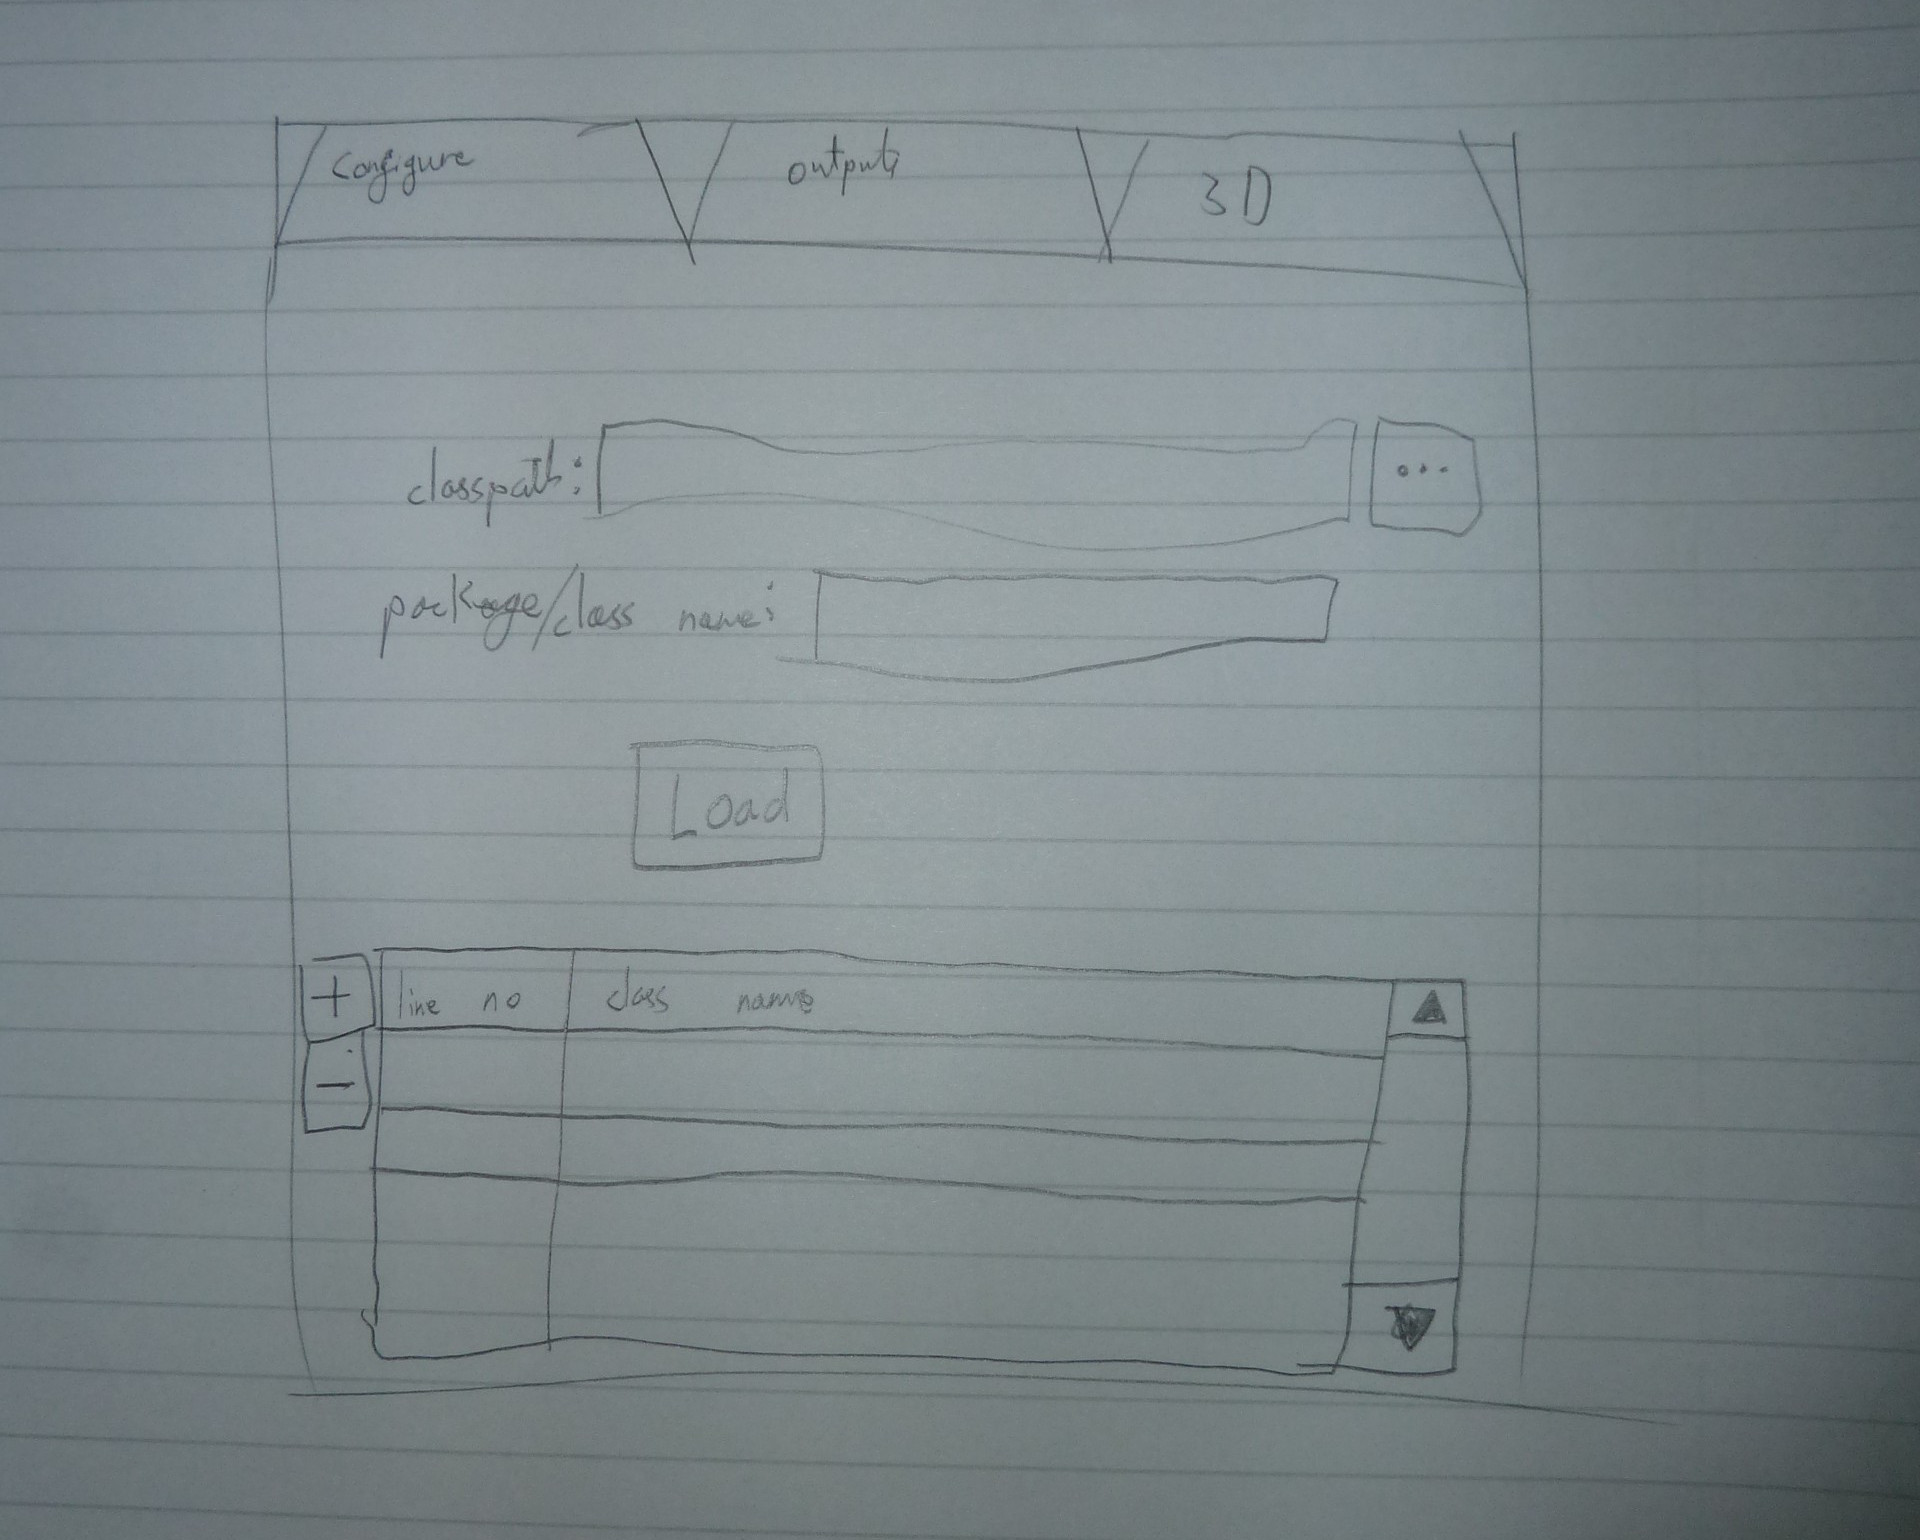
\includegraphics[width=200px]{images/paper_prototype.JPG}
        \caption{Paper Prototypes}
\end{figure}

\subsection{Spikes}

Spike is a technique which allows developers tackle technical problems at early stage including using new technology. It refers to short time-boxed pieces of research, normally of technical nature, to provide the team with just enough information to continue.

We set the starting point as choosing an appropriate game engine, then learnt and tested it and finally decide whether to accept it. After first round filtering, we chose Unity, which looks quite simple at a glance, but after testing it, we found that we needed to learn C{\#}/javascript and it is not easy to hook up the debugger wrote in Java. We realized that a game engine with built-in IDE is not what we wanted, a better option should allow us to build the game directly either from scratch or in Java IDE such as Eclipse. This brought Java 3D to our attention. The main drawback of Java 3D is that Java 3D is a heavyweight component. In general lightweight and heavyweight component’s don’t mix very well so it may prove tricky to link together the windows in our Java swing application with the elements of our 3D visualisation. This said, its high-level, object oriented view of 3D graphics makes it straight forward to learn and as it is optimized for speed where possible it is a good fit for our application. We also tested JMonkeyEngine 3 which can be set up in Eclipse and is simpler than Java 3D with equal benefits. As a result, our final decision is JME 3. 

Although some might not call it a spike as there was no code to integrate with, we used a similar technique at the beginning of the project when writing the debugger. A JVM provides a standard interface, the Java Platform Debugger Architecture, which allows external processes to inspect VM state. This is split into two levels, the high-level Java Debugger Interface for use in Java programs and low-level Java Virtual Machine Tools Interface for use with native code. We wanted already intended to code the project in Java and thought a high level interface would be more appropriate than a low level one. We ensured we would be able to use the Java Debugger Interface (JDI) by modifying an example program it ships with (“trace”) to do the tasks we wanted -- adding breakpoints, inspecting the stack and finding the objects referenced by a given object. Once we established the JDI was straightforward to use we started afresh and rewrote the debugger in a more mindful fashion.

This exercise was very helpful as it meant that we weren’t bogged down by implementation details when writing the final debugger code; any misunderstandings had already been cleared. As a result we could concentrate on program architecture.

\subsection{Impact Mapping}

We do not build products independently. Our product should be built as customers desired.  Impact mapping helps us focus on the core features needed in our project and prevents us spending time on unrealistic tasks. We make impact mapping by making assumptions and our customers can decide if the prioritisation matches. From the impact map, each deliverable we plan to make should have corresponding impact.  

\begin{figure}[h]
        \centering
        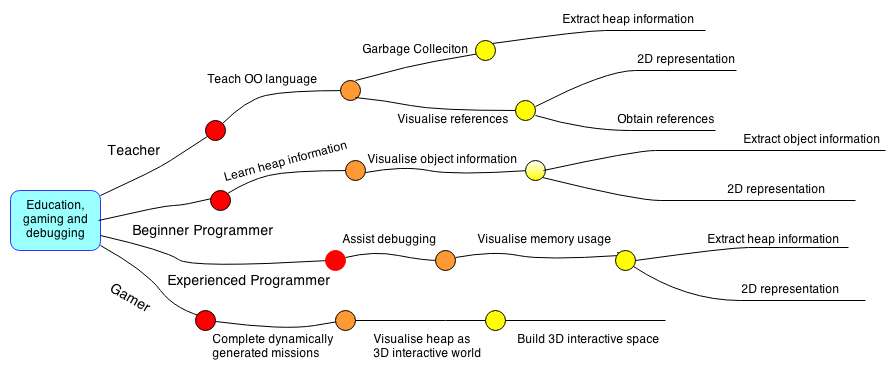
\includegraphics[width=350px]{images/Impact_mapping.png}
        \caption{Impact Mapping}
\end{figure}

The map above shows the dynamic relation between customers and developers. The goal of the project is in the blue box. The first branch specifies ‘actors’ in the project. The second level are the impacts we are achieving and the bottom level shows what we can do to make the expected impacts. 

\section{Feedback}

Our product should result in a usable tool for both lecturers and students. To achieve this, its important that we regularly gather feedback as part of our iterative development practice so that we can produce a product which is useful and usable. Once all the components of the project come together, we can extend our testing efforts to our other stakeholders, in order to gain further insights for improvement. 

We plan to collect feedback on our product using both formative and heuristic evaluation techniques. An example of formative evaluation we plan to use is the focus group\textsuperscript{\cite{focus}}. By having actual potential users test our project we are able to gain a new understanding of the product with a fresh set of eyes and consider things from a new angle. However, by approaching a set of students in this manner, it has the con that the group discussion can sometimes be hard to manage and certain points of interest can be lost in the general flow of a conversation. To facilitate this focus group we plan to present a number of questions for them to work through and discuss. Here are some examples:
\begin{itemize}

  \item How easy was it to use without asking questions?
  \item Was the output clear?
  \item How attractive is the product on a scale of 1 - 10
  \item Is there anything you’d like to see in the product? 
  \item Was navigating the 3D space as you expected, or did you encounter problems? 
  \item How easy was it to begin debugging a program? (Scale of 1 - 10) 
  \item Did the tool help you understand how the heap of objects has been organised? 
      
\end{itemize}
We were advised by our supervisor to test our questionnaire on a couple of people without using their results, just to sanity check the survey, before allowing more people to answer it. We feel this is a good idea to help improve the integrity of our results.

To compliment this we also plan to perform some heuristic evaluation. Jacob Nielsons has written extensively on this subject and we plan to work through the ten usability heuristics for design that he presents\textsuperscript{\cite{heuristic}} and apply them to our product. Whilst it presents no new outlook on the product, given our familiarity with the piece, with these guidelines we will be able to quickly identify specific points about the project and how to improve them relative to the feedback we also get from the formative evaluation. 

To further improve on the user experience of our tool, we could try to record some quantitative data on how users interact with the product. These would include the amounts of idle time between mouse clicks, recording the path of a user through the program, where they get stuck and perhaps even using some A/B testing to try different program layouts. This data would allow us to see areas that would need improvements, but the disadvantage is having to actually implement the mechanisms for collecting these analytics, so it is unlikely that we will use this particular technique to gather feedback from potential users. However, after the project is completed, we could use it for further improvements.

\section{Supervisor Discussion}

We have already been gathering feedback from our supervisor, who was able to attempt to use our newly designed GUI for the debugger tool, without prior experience and with little understanding of what he was trying to achieve. We took notes on his experience as well as comments he made during the process, which we will be implementing soon. He pointed out to use a few areas where things were poorly labelled and would allow use to improve the clarity of the GUI, hopefully leading to a better user experience.

\begin{thebibliography}{9}

\bibitem{eight}
  Christiaan Verwijs, 
  \emph{8 Useful Strategies for Splitting Large User Stories},
  \\ http://www.christiaanverwijs.nl/post/2013/05/17/8-useful-strategies-for-splitting-large-user-stories-{\%}28and-a-cheatsheet{\%}29.aspx

\bibitem{focus} 
  Evaluation Toolbox, 
  \emph{Focus Group},
  \\ http://evaluationtoolbox.net.au/index.php?option=com{\_}content{\&}view=article{\&}id=32{\&}Itemid=140

\bibitem{mikeadv} 
  Mike Cohn, 
  \emph{Advantages of User Stories for Requirements}, 
  \\ http://www.mountaingoatsoftware.com/articles/advantages-of-user-stories-for-requirements

\bibitem{heuristic} 
  Jacob Nielson, 
  \emph{10 Usability Heuristics for User Interface Design},
  \\ http://www.nngroup.com/articles/ten-usability-heuristics/

\bibitem{proto}
  Jacob Nielson, 
  \emph{Paper Prototyping: Getting User Data Before You Code},
  \\ http://www.nngroup.com/articles/paper-prototyping/

\bibitem{internal} 
  Donna Earl, 
  \emph{What Is Internal Customer Service? A Definition and Case Study}
  \\ http://www.donnaearltraining.com/Articles/InternalCustomerService.html

\bibitem{internal2}
  Chris Joseph, 
  \emph{What Is an Internal Customer {\&} a External Customer?},
  \\ http://smallbusiness.chron.com/internal-customer-external-customer-11698.html

\bibitem{stakeholder} 
  Rachel Thompson, 
  \emph{Stakeholder Analysis: Winning Support for Your Projects},
  \\ http://www.mindtools.com/pages/article/newPPM{\_}07.htm

\end{thebibliography}

\end{document}
